\documentclass[5pt]{article}

%packages

\usepackage{titlesec}
\usepackage{titling}
\usepackage[margin=0.5in] {geometry}
\usepackage{multicol}
\usepackage{hyperref}
\usepackage{graphicx}


%section

\titleformat{\section}
{ \bfseries \uppercase}
{\hspace{-.25in}\thesection}
{0em}
{. }[\titlerule]


%sub Section

\titleformat{\subsection}
{\bfseries\large}
{$\bullet$}
{0em}
{ }

%sub Sub Section

\titleformat{\subsubsection}[runin]
{\bfseries}
{}
{0em}
{-}  

\titlespacing{\subsubSection}
{0em}{0em}{0em}


%make titile

\renewcommand{\maketitle}{
\begin{center}
{\LARGE\bfseries
\theauthor}

\vspace{.25em}
\line(1,0){250}
\end{center}
\begin{multicols}{2}
\noindent
%address
Fl.No. 11/A,\\
Hariangan Society,\\
Near New Life Hospital,\\
Gurudwara Chowk,\\
Akurdi,Pune -411044\\

\columnbreak
\begin{flushright}
Contact: +91-7798497481\\
E-mail Id: aditya.bichave@gmail.com\\
Github: \url{https://github.com/Aditya-Bichave}
\end{flushright}
\noindent
\hspace{10em}
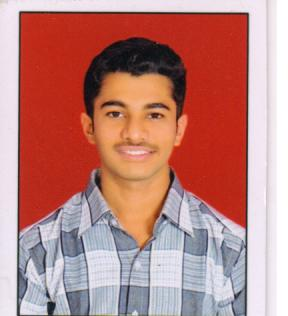
\includegraphics[width = 6em]{Aditya.jpg}

\end{multicols}



}





















\begin{document}

\title{Resume}
\author{Aditya Bichave}
\maketitle

\section{Objective}

To seek a challenging position as a Machine Learning Engineering with an organization of repute, where I can utilize my skills and knowledge of Computer Science concepts and advance technologies like Deep Learning, Image processing.

\section{Education}

\begin{tabular}[8pt]{| c | c | c | c | c |}
\hline
	Degree & College/School & University & passing year & Pass Percentage\\
\hline
	B.E Computer Engineering & Pimpri Chinchawad College of Engineering ,Pune & SPPU & 2021 & -- \\
\hline
	First Year & Pimpri Chinchawad College of Engineering ,Pune & SPPU & 2018 & 9.48 CGPA \\
\hline
	H.S.C & Ashoka Universal School and Jr.College,Nashik & ISC & 2017 & 83.60 \\
\hline
	S.S.C & Sacred Heart Convent High School, Nashik & S.S.C & 2015 & 91.00\\
\hline
\end{tabular} 

\section{Projects}
	\begin{enumerate}
		\item E-yantra Project Based Competition: Project on Animal home coming. Where animals and Habitates are extracted from image and than image is feed to deep learning model which classifies the animal and maps the animal to there habitate. This data is later transfered to a bot which searches the minimum path for reaching to animal, Pick the animal and place it in respective habitate.
			\begin{itemize}
			\item Languages Used: Python , C, C++
			\item Technologies Used: PyTorch , Atmega 2560, OpenCV, Atmel Studio, 
			
			\end{itemize}
		\item Android Attendace App with Firebase support: Android app which helps manage College Attendace of students.
			\begin{itemize}
			\item Languages Used: Java, XML.
			\item Technologies Used: Android Studio, Firebase by Google. 
			
			\end{itemize}
		\item Airship shooting Game:  A Game based on python.  where player has to control airship movement and the firing way of the airship. Player with maximum Score wins.
			\begin{itemize}
			\item Languages Used: Python.
			\item Technologies Used: PyGame , Visual Studio. 
			
			\end{itemize}
  
	\end{enumerate}


\section{Training \& Internship}
\subsection{Training:}
\begin{enumerate}
\item Project based Learning By Eyantra,IIT Bombay.
\item Hands On Training For Internet Of things and Robotics by Microsoft and IIT bombay.
\item Hands On Training For Android by Skylabs and IIT hyderabad.
\item Artifical Intelligence and Machine Learning Workshop At PCCOE, Pune. 
\end{enumerate}
\subsection{Internship:}
NONE

\section{Research publications}
	NONE.
\section{Technical Skills}
	\subsection{Languages:}
		\subsubsection{Programming Languages: }
			C, C++, Python, Java.
		\subsubsection{Markup Languages:}
			HTML,CSS,XML
		\subsubsection{Tools}
			PyTorch,Tensorflow,Keras, Sklearn, OpenCV,Android Studio,Atmel Studio,Arduino, Google Colab

\section{Soft Skills}
	\begin{multicols}{3}
	\begin{itemize}
	\item Confident \\
 	\item Problem Solving\\
	\item Motivated\\ 
	\columnbreak
	\item Curious\\
	\item Persistent \\
	\item Teamwork\\
	\columnbreak
	\item Self-managment\\
	\item Leadership
	\end{itemize}
	\end{multicols}


\section{Extra-curricular Activities}
\begin{enumerate}
\item Is a member of Compter Engineering Student Association and ACM Student Chapter at Computer Depatment,PCCOE, Pune.
\item Currently working with 72 people as Volunteer at Training and Placement Cell, PCCOE.
\item Worked as Co-ordinator For Spectrum, an event organized by PCCOE.  A massive crowd of around 500 - 700 people \& students all over pune gathered for participating in various competition .
\item Worked with Training and placement Cell, PCCOE for handling various Job Drives including both on-campus and off-campus drives.
\end{enumerate}


\section{co-curricular activities}
\begin{enumerate}
\item Secure 3rd place in C - Coder event PICT,Pune.
\item Currently enrolled in Core Java.
\item Completed Python Courses , Sympy,pygame, 
\item Completed Coursra Machine Learning course By Andrew NG. 
\item Curently pursuing PyTorch tutorials from Pytorch official website, also Referring to various other resourses for accumalating more knowledge on Deep Learning.
\end{enumerate}


\section{Personal Details} 
\begin{itemize}

\item{Father's Name: Anand Bichave}
\item{Mother's Name: Rashmi Bichave}
\item{Sex: Male}
\item{Date Of Birth: 9th April, 1999}
\item{Nationality: Indian}
\item{Marital Status: Single}

\end{itemize}

%Ref
\noindent
\textbf{Reference}
\\
Mrs Sangita Patil\\
E-mail id: sapatil1912@gmail.com\\

%decleraion
\noindent
\textbf{Declaration}
\\
I hereby declare that above-mentioned information is correct to the best of my knowledge and belief\\
\\
Place: Pune\\
Date: 17 April ,2019





\end{document} 